\section{背景}

\begin{frame}{LD Cycleによる生体リズムの研究}
    \begin{minipage}{0.49\linewidth}
        時差ぼけの研究:
        \begin{itemize}
            \item 繰り返しの時差ぼけや交代制勤務は、心臓疾患や代謝不全などの生活習慣病のリスクを高める.
            \item 概日リズムに対する環境の光暗サイクルの影響を研究するためにLDサイクルが使われることがある.\begin{itemize}
                \item 光・暗闇12時間ずつのサイクルを8時間進めたり遅らせたりしてマウスの行動リズムを研究する.
            \end{itemize}
        \end{itemize}
    \end{minipage}
    \begin{minipage}{0.5\linewidth}
        \begin{itemize}
            \item LD Cycleは周期的な挙動を持つが,外力を加えることでカオス的に振る舞うことがある.
            \item カオスを含む非線形力学系の予測ができれば,未来における概日リズムをより詳細に把握できる.
        \end{itemize}
        \begin{figure}
            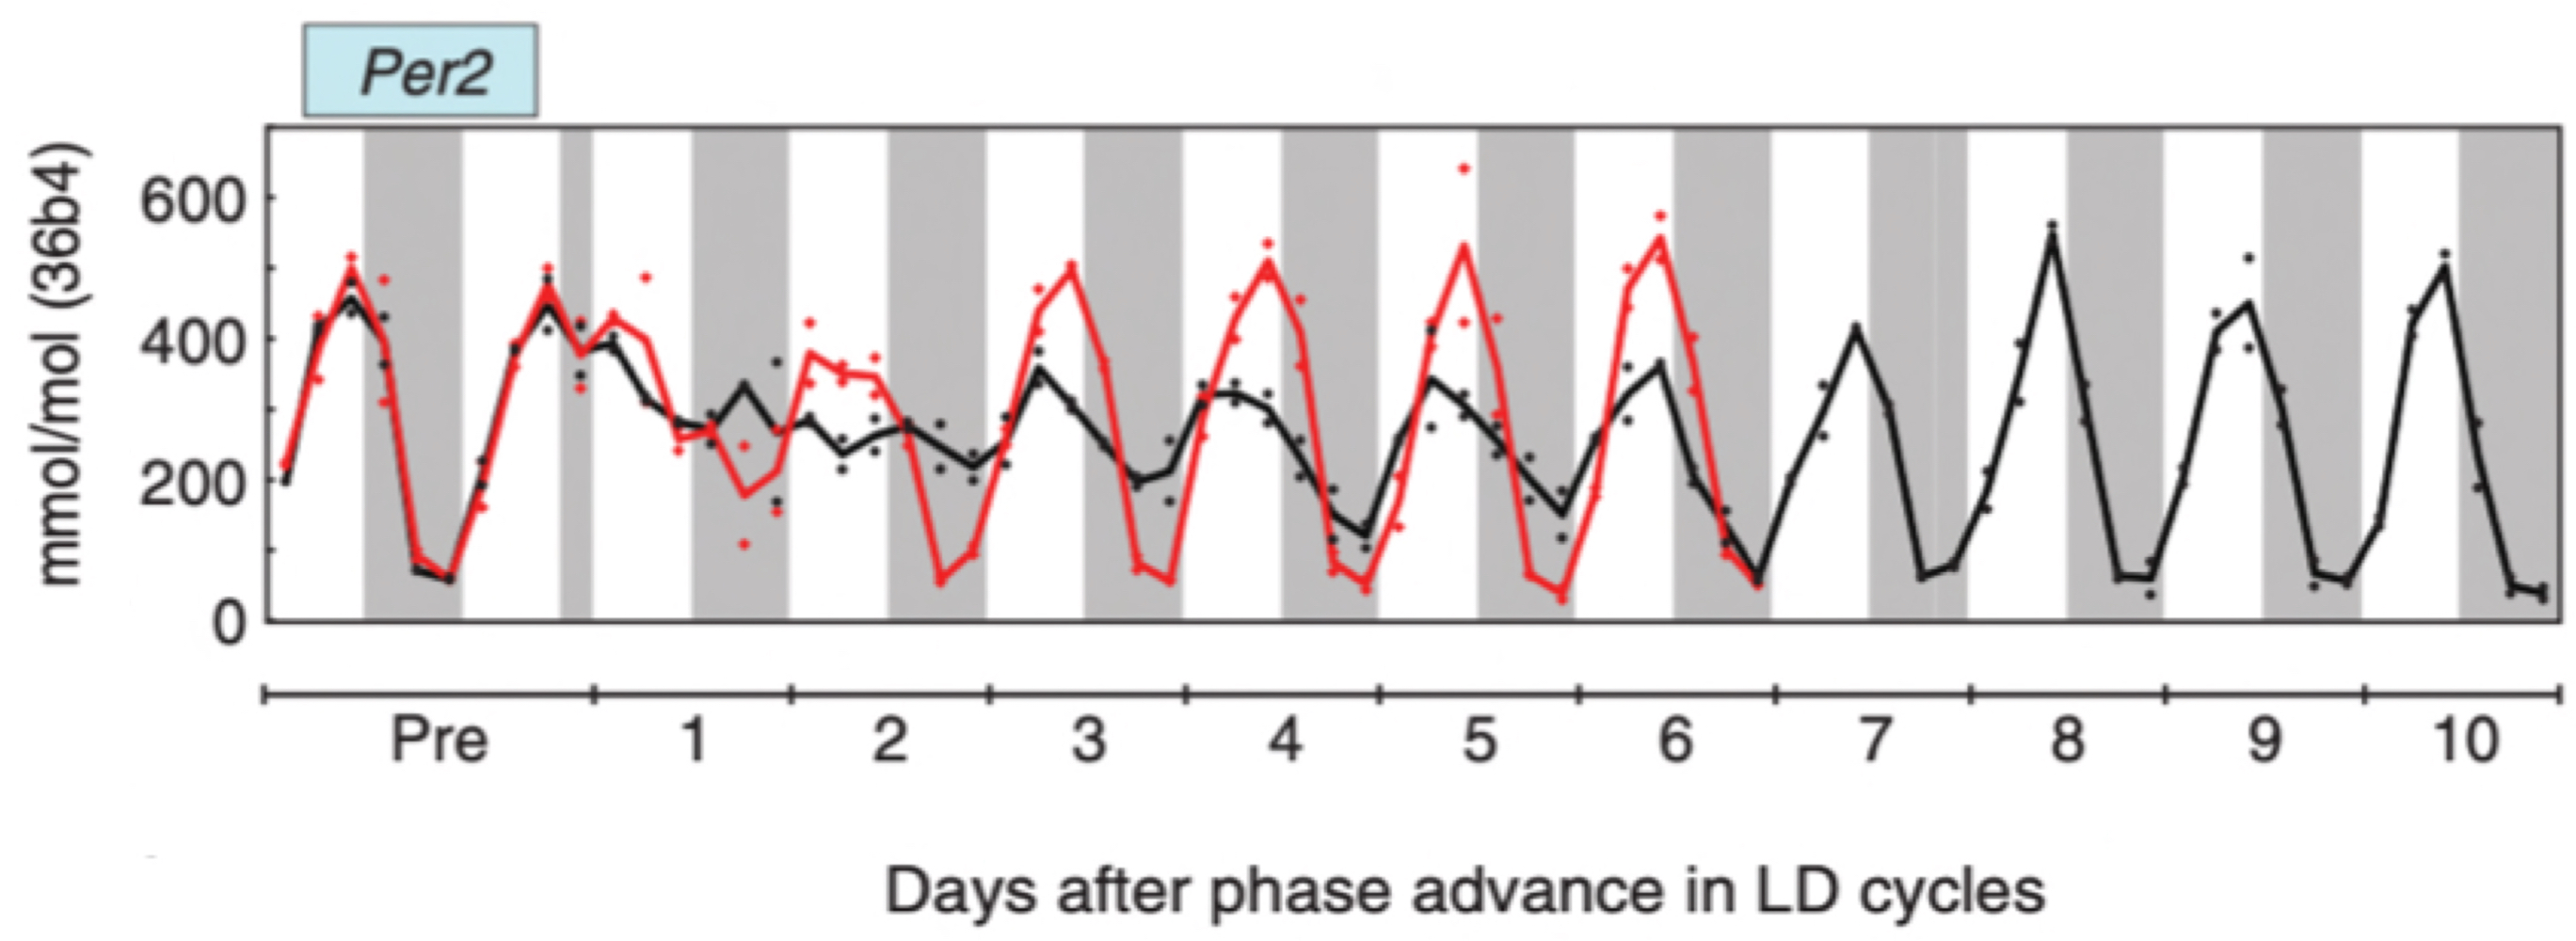
\includegraphics[width=0.75\textwidth]{Fig/Jetlag.png}
            \caption{Day 1に8時間のJet Lagを受けた時のマウスの Per2 の推移}
            \label{jetlag} 
        \end{figure}    
    \end{minipage}
\end{frame}

\begin{frame}{レザバーを用いたカオス時系列の未来予測}
    
    \begin{itemize}
        \item 現実の問題は非線形で,高次元・複雑→完全な数理モデルを作ることは難しい.
        \item 非線形力学システムの未来予測は一般に困難
        \begin{itemize}
            \item 特にカオスの場合は初期値鋭敏性により,(外部からの干渉も影響し)不完全な数理モデルでは予測に用いにくい.
        \end{itemize}
        \item Reservoir Computer を用いて高い精度の予測が可能
        \begin{block}{Reservoir Computer}
            内部にランダムニューラルネットワーク(Reservoir)を持つRecurrent Neural Networkの手法.Backpropagationが不必要・出力層のみの学習で計算効率が良い. 
        \end{block}    
    \end{itemize}      
\end{frame}
